\documentclass[11pt]{exam}
\usepackage[margin=1in]{geometry}
\usepackage{tasks}
\usepackage{amsfonts, amsmath, amssymb, amsthm}
\usepackage{mathtools}
\usepackage{enumerate}
\usepackage{listings}
\usepackage{colortbl}
\usepackage{float}
\usepackage[colorlinks,linkcolor=blue]{hyperref}

% in order to compile this file you need to get 'header.tex' from
% Canvas and change the line below to the appropriate file path
%%% theorems

\theoremstyle{plain}            % following are "theorem" style
\newtheorem{theorem}{Theorem}[section]
\newtheorem{lemma}[theorem]{Lemma}
\newtheorem{corollary}[theorem]{Corollary}
\newtheorem{proposition}[theorem]{Proposition}
\newtheorem{claim}[theorem]{Claim}
\newtheorem{fact}[theorem]{Fact}
\newtheorem{openproblem}[theorem]{Open Problem}

\theoremstyle{definition}       % following are def style
\newtheorem{definition}[theorem]{Definition}
\newtheorem{conjecture}[theorem]{Conjecture}
\newtheorem{example}[theorem]{Example}
\newtheorem{protocol}[theorem]{Protocol}
\newtheorem{exercise}[theorem]{Exercise}

\theoremstyle{remark}           % following are remark style
\newtheorem{remark}[theorem]{Remark}
\newtheorem{note}[theorem]{Note}
%\newtheorem*{solution}{Solution}

%%% special sets
\newcommand{\bit}{\ensuremath{\{0,1\}}}
\newcommand{\bitt}{\ensuremath{\{-1,1\}}}
\newcommand{\ball}{\ensuremath{\mathcal{B}}}
\newcommand{\sph}{\ensuremath{\mathbb{S}}}
\newcommand{\odisc}[2]{\ensuremath{D(#1, #2)}}
\newcommand{\cdisc}[2]{\ensuremath{\bar{D}(#1, #2)}}
\newcommand{\emp}{\varnothing}

% constants
\newcommand{\E}{\ensuremath{\mathrm{e}}}
\newcommand{\I}{\ensuremath{\mathrm{i}}}
\newcommand{\Id}{\ensuremath{\mathrm{I}}}
\newcommand{\paulix}{\ensuremath{\mathrm{X}}}
\newcommand{\pauliy}{\ensuremath{\mathrm{Y}}}
\newcommand{\pauliz}{\ensuremath{\mathrm{Z}}}

% font for general-purpose algorithms
\newcommand{\algo}[1]{\ensuremath{\mathsf{#1}}}
% font for general-purpose computational problems
\newcommand{\problem}[1]{\ensuremath{\mathsf{#1}}}
% font for complexity classes
\newcommand{\class}[1]{\ensuremath{\mathsf{#1}}}

% asymptotics
\DeclareMathOperator{\poly}{poly}
\DeclareMathOperator{\polylog}{polylog}
\DeclareMathOperator{\negl}{negl}
\DeclareMathOperator{\bigO}{O}
\DeclareMathOperator{\litO}{o}
\DeclareMathOperator{\Otil}{\tilde{O}}
\DeclareMathOperator{\Ostar}{O^*}

%%% "LEFT-RIGHT" PAIRS OF SYMBOLS

% inner product
\DeclarePairedDelimiter\inner{\langle}{\rangle}
% absolute value
\DeclarePairedDelimiter\abs{\lvert}{\rvert}
% a set
\DeclarePairedDelimiter\set{\{}{\}}
% parens
\DeclarePairedDelimiter\parens{(}{)}
% tuple, alias for parens
\DeclarePairedDelimiter\tuple{(}{)}
% square brackets
\DeclarePairedDelimiter\bracks{[}{]}
% rounding off
\DeclarePairedDelimiter\round{\lfloor}{\rceil}
% floor function
\DeclarePairedDelimiter\floor{\lfloor}{\rfloor}
% ceiling function
\DeclarePairedDelimiter\ceil{\lceil}{\rceil}
% length of some vector, element
\DeclarePairedDelimiter\length{\lVert}{\rVert}
% "lifting" of a residue class
\DeclarePairedDelimiter\lift{\llbracket}{\rrbracket}
\DeclarePairedDelimiter\len{\lvert}{\rvert}
% bra-kets
\DeclarePairedDelimiter\bra{\langle}{\rvert}
\DeclarePairedDelimiter\ket{\lvert}{\rangle}
\newcommand{\braket}[2]{\ensuremath{\langle #1 \vert #2 \rangle}}
\newcommand{\ketbra}[2]{\ensuremath{\lvert #1 \rangle \langle #2 \rvert}}

%%% spacing

\newcommand{\ws}{\hspace{1pt}}
\newcommand{\wws}{\hspace{2pt}}
\newcommand{\hs}{\hspace{4pt}}
\newcommand{\hhs}{\hspace{8pt}}
\newcommand{\hhhs}{\hspace{12pt}}

%%% LISTS

\newcommand{\oneto}{1, \ldots,}
\newcommand{\onetop}{1 \cdots,}
\newcommand{\zeroto}{0, \ldots,}
\newcommand{\zerotop}{0 \cdots,}
\newcommand{\perm}[1]{\mathbf{(#1)}}
\newcommand{\permv}[1]{(#1)}
\newcommand{\varind}[2]{#1_1, \ldots, #1_#2}
\newcommand{\varindz}[2]{#1_0, \ldots, #1_#2}
\newcommand{\varindp}[2]{#1_1 \cdots #1_#2}
\newcommand{\varindpz}[2]{#1_0 \cdots #1_#2}
\newcommand{\seq}[2]{(#1_#2)_{#2=1}^\infty}
\newcommand{\seqz}[2]{(#1_#2)_{#2=0}^\infty}

%%% MATH OPERATORS

%\DeclareMathOperator{\pr}{\mathbf{P}}
%\DeclareMathOperator{\ex}{\mathbf{E}}
\DeclareMathOperator{\pr}{P}
\DeclareMathOperator{\ex}{E}
\DeclareMathOperator{\Span}{Span}
\DeclareMathOperator{\tr}{Tr}
\DeclareMathOperator{\supp}{Supp}
\DeclareMathOperator{\im}{Im}
\DeclareMathOperator{\var}{var}
\DeclareMathOperator{\vol}{vol}
\DeclareMathOperator{\sign}{sign}
\DeclareMathOperator{\dkl}{D_{KL}}
\DeclareMathOperator{\entr}{H}
\DeclareMathOperator{\fid}{F}
\DeclareMathOperator{\dist}{D}
\DeclareMathOperator{\ad}{ad}

% hats

\newcommand{\fhat}{\ensuremath{\hat{f}}}
\newcommand{\phat}{\ensuremath{\hat{p}}}
\newcommand{\that}{\ensuremath{\hat{t}}}

%%% BLACKBOARD SYMBOLS

% \newcommand{\C}{\ensuremath{\mathbb{C}}}
\newcommand{\D}{\ensuremath{\mathbb{D}}}
\newcommand{\F}{\ensuremath{\mathbb{F}}}
% \newcommand{\G}{\ensuremath{\mathbb{G}}}
\newcommand{\J}{\ensuremath{\mathbb{J}}}
\newcommand{\N}{\ensuremath{\mathbb{N}}}
\newcommand{\Q}{\ensuremath{\mathbb{Q}}}
\newcommand{\R}{\ensuremath{\mathbb{R}}}
\newcommand{\T}{\ensuremath{\mathbb{T}}}
\newcommand{\Z}{\ensuremath{\mathbb{Z}}}
\newcommand{\QR}{\ensuremath{\mathbb{QR}}}

% sets in calligraphic type

\newcommand{\calD}{\ensuremath{\mathcal{D}}}
\newcommand{\calF}{\ensuremath{\mathcal{F}}}
\newcommand{\calG}{\ensuremath{\mathcal{G}}}
\newcommand{\calH}{\ensuremath{\mathcal{H}}}
\newcommand{\calI}{\ensuremath{\mathcal{I}}}
\newcommand{\calL}{\ensuremath{\mathcal{L}}}
\newcommand{\calN}{\ensuremath{\mathcal{N}}}
\newcommand{\calP}{\ensuremath{\mathcal{P}}}
\newcommand{\calS}{\ensuremath{\mathcal{S}}}
\newcommand{\calX}{\ensuremath{\mathcal{X}}}
\newcommand{\calY}{\ensuremath{\mathcal{Y}}}

% matrices and vectors

\newcommand{\matA}{\ensuremath{\mathbf{A}}}
\newcommand{\matB}{\ensuremath{\mathbf{B}}}
\newcommand{\matC}{\ensuremath{\mathbf{C}}}
\newcommand{\matD}{\ensuremath{\mathbf{D}}}
\newcommand{\matE}{\ensuremath{\mathbf{E}}}
\newcommand{\matF}{\ensuremath{\mathbf{F}}}
\newcommand{\matG}{\ensuremath{\mathbf{G}}}
\newcommand{\matH}{\ensuremath{\mathbf{H}}}
\newcommand{\matI}{\ensuremath{\mathbf{I}}}
\newcommand{\matJ}{\ensuremath{\mathbf{J}}}
\newcommand{\matK}{\ensuremath{\mathbf{K}}}
\newcommand{\matL}{\ensuremath{\mathbf{L}}}
\newcommand{\matM}{\ensuremath{\mathbf{M}}}
\newcommand{\matN}{\ensuremath{\mathbf{N}}}
\newcommand{\matO}{\ensuremath{\mathbf{O}}}
\newcommand{\matP}{\ensuremath{\mathbf{P}}}
\newcommand{\matQ}{\ensuremath{\mathbf{Q}}}
\newcommand{\matR}{\ensuremath{\mathbf{R}}}
\newcommand{\matS}{\ensuremath{\mathbf{S}}}
\newcommand{\matT}{\ensuremath{\mathbf{T}}}
\newcommand{\matU}{\ensuremath{\mathbf{U}}}
\newcommand{\matV}{\ensuremath{\mathbf{V}}}
\newcommand{\matW}{\ensuremath{\mathbf{W}}}
\newcommand{\matX}{\ensuremath{\mathbf{X}}}
\newcommand{\matY}{\ensuremath{\mathbf{Y}}}
\newcommand{\matZ}{\ensuremath{\mathbf{Z}}}
\newcommand{\matzero}{\ensuremath{\mathbf{0}}}

\newcommand{\veca}{\ensuremath{\mathbf{a}}}
\newcommand{\vecb}{\ensuremath{\mathbf{b}}}
\newcommand{\vecc}{\ensuremath{\mathbf{c}}}
\newcommand{\vecd}{\ensuremath{\mathbf{d}}}
\newcommand{\vece}{\ensuremath{\mathbf{e}}}
\newcommand{\vecf}{\ensuremath{\mathbf{f}}}
\newcommand{\vecg}{\ensuremath{\mathbf{g}}}
\newcommand{\vech}{\ensuremath{\mathbf{h}}}
\newcommand{\veck}{\ensuremath{\mathbf{k}}}
\newcommand{\vecm}{\ensuremath{\mathbf{m}}}
\newcommand{\vecp}{\ensuremath{\mathbf{p}}}
\newcommand{\vecq}{\ensuremath{\mathbf{q}}}
\newcommand{\vecr}{\ensuremath{\mathbf{r}}}
\newcommand{\vecs}{\ensuremath{\mathbf{s}}}
\newcommand{\vect}{\ensuremath{\mathbf{t}}}
\newcommand{\vecu}{\ensuremath{\mathbf{u}}}
\newcommand{\vecv}{\ensuremath{\mathbf{v}}}
\newcommand{\vecw}{\ensuremath{\mathbf{w}}}
\newcommand{\vecx}{\ensuremath{\mathbf{x}}}
\newcommand{\vecy}{\ensuremath{\mathbf{y}}}
\newcommand{\vecz}{\ensuremath{\mathbf{z}}}
\newcommand{\veczero}{\ensuremath{\mathbf{0}}}
\newcommand{\vecone}{\ensuremath{\mathbf{1}}}

\newcommand{\vecell}{\ensuremath{\boldsymbol\ell}}
\newcommand{\vecalpha}{\ensuremath{\boldsymbol\alpha}}
\newcommand{\vecbeta}{\ensuremath{\boldsymbol\beta}}
\newcommand{\veceta}{\ensuremath{\boldsymbol\eta}}
\newcommand{\vecmu}{\ensuremath{\boldsymbol\mu}}
\newcommand{\vecphi}{\ensuremath{\boldsymbol\phi}}
\newcommand{\vecsigma}{\ensuremath{\boldsymbol\sigma}}
\newcommand{\vectheta}{\ensuremath{\boldsymbol\theta}}
\newcommand{\vecxi}{\ensuremath{\boldsymbol\xi}}

%%% misc

\newcommand{\ind}{\ensuremath{\mathbf{1}}}

\newcommand{\congmod}[3]{#1 \equiv #2 \textrm{ modulo } #3}

\newcommand{\dee}{\,\mathrm{d}}
\newcommand{\de}{\mathrm{d}}
\newcommand{\dx}{\,\mathrm{d} x}

\newcommand{\ol}{\overline}
\newcommand{\inv}[1]{\ensuremath{#1^{-1}}}
\newcommand{\tsp}[1]{\ensuremath{#1^{\top}}}


\newcommand{\eps}{\varepsilon}
\newcommand{\ph}{\varphi}

\newcommand{\Ra}{\Rightarrow}
\newcommand{\Lra}{\Leftrightarrow}
\newcommand{\rsqa}{\rightsquigarrow}

\newcommand{\trl}{\triangleleft}
\newcommand{\trr}{\triangleright}

\newcommand{\func}[3]{#1: #2 \to #3}
\newcommand{\dd}[1]{\frac{\mathrm{d}}{\mathrm{d}#1}}
\newcommand{\ptl}[1]{\frac{\partial}{\partial #1}}
\newcommand{\prtl}[2]{\frac{\partial #1}{\partial #2}}

\newcommand{\matrixtt}[4]{
  \begin{pmatrix*}[r]
        #1 & #2 \\
        #3 & #4
    \end{pmatrix*}
}

%%% for homework and section notes

\newcommand{\commonheader}[2]{
    \pagestyle{headandfoot}
    \setlength{\headheight}{26pt}
    \setlength{\headsep}{30pt}

    \header
        {\small{\textbf{VE281: Data Structures and Algorithms}} \\ \footnotesize{\textbf{UM-SJTU Joint Institute, FA2022}}}
        {#1}
        {#2}

    \firstpageheadrule
    \runningheadrule

    \footer
        {}
        {\thepage}
        {}
}

\newcommand{\hwheader}{
    \commonheader
        {\textbf{Homework \hwnum}}
        {\small \textbf{Due at \duedate}}
}

\newcommand{\hwslnheader}{
    \commonheader
    	{}
        {\textbf{Solutions to Homework \hwnum}}
    \printanswers
}

\newcommand{\notesheader}{
    \commonheader
        {\Large \textbf{Section Notes \sectionnum}}
    	{}
}

\newcommand{\hint}[1]{
\emph{Hint}: #1
}

% for effort questions
\let\Eitem=\relax
\def\effortE{\textbf{E}~}
\makeatletter
\def\Eitem{%
    \expandafter\let\expandafter\originallabel\csname labelenum\romannumeral\@enumdepth\endcsname
    \expandafter\def\csname labelenum\romannumeral\@enumdepth\expandafter\endcsname\expandafter{%
        \expandafter\effortE\originallabel}%
    \item
    \expandafter\let\csname labelenum\romannumeral\@enumdepth\endcsname\originallabel
}
\makeatother

\allowdisplaybreaks

\geometry{left=2.5 cm,right=2.5 cm,top=2.5 cm,bottom=2.5 cm}
%\pagestyle{fancy}
\definecolor{mygreen}{rgb}{0,0.6,0}  
\definecolor{mygray}{rgb}{0.5,0.5,0.5}
\definecolor{mymauve}{rgb}{0.58,0,0.82} 
\definecolor{background}{rgb}{0.963,0.963,0.963}

\definecolor{codegreen}{rgb}{0,0.6,0}
\definecolor{codegray}{rgb}{0.5,0.5,0.5}
\definecolor{codepurple}{rgb}{0.58,0,0.82}
\definecolor{backcolour}{rgb}{0.95,0.95,0.92}

\lstdefinestyle{mystyle}{
    backgroundcolor=\color{backcolour},   
    commentstyle=\color{codegreen},
    keywordstyle=\color{magenta},
    numberstyle=\tiny\color{codegray},
    stringstyle=\color{codepurple},
    basicstyle=\ttfamily\footnotesize,
    breakatwhitespace=false,         
    breaklines=true,                 
    captionpos=b,                    
    keepspaces=true,                 
    numbers=left,                    
    numbersep=5pt,                  
    showspaces=false,                
    showstringspaces=false,
    showtabs=false,                  
    tabsize=2,
    language=c++
}

\lstset{style=mystyle}
\newcommand{\hwnum}{4}
\newcommand{\duedate}{11:59pm, November 13th}

%\notesheader
\hwheader   % header for homework
%\hwslnheader   % header for homework solutions

% Comment the following line in order to hide solutions.
% Uncomment the line to show solutions written inside of
% LaTeX solution environments like:
%   \begin{solution}
%     My solution.
%   \end{solution}.
\printanswers

\begin{document}
\setlength{\parindent}{0pt}
\section*{Before you start:}

\subsection*{Homework Files}
You can download the starter files for coding as well as this \textit{tex} file (you only need to modify \textit{homework4.tex}) on canvas and do your homework with latex. 
Or you can scan your handwriting, convert to pdf file, and upload it to canvas before the due date. If you choose to write down your answers by hand, you can directly download the pdf file on canvas which provides more blank space for solution box.\\

\subsection*{Submission Form}
A pdf file as your solution named as VE281\_HW4\_[Your Student ID]\_[Your name].pdf uploaded to canvas


Estimated time used for this homework: \textbf{3-4 hours.}
\\\\


\newpage
\section*{0\quad Student Info}
Your name and student id:
\begin{solution}
% Write your answer here
\end{solution}

\section{Basic knowledge of AVL treec}
There are some questions about the basic knowledge of AVL tree.
\begin{enumerate}
\item Which of the following binary search trees is an AVL tree?
\begin{figure}[H]
     \centering
    \subfigure[A]{
       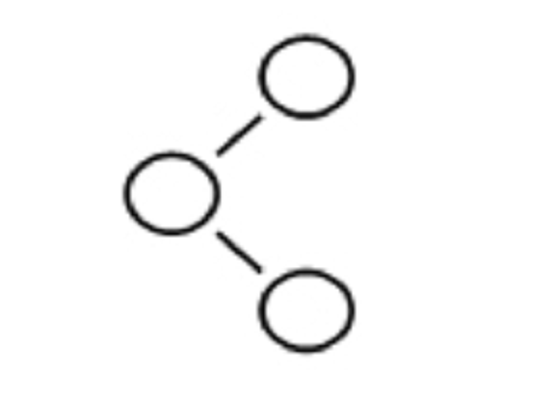
\includegraphics[scale=1]{a.PNG}}
     \hspace{0.5in} 
     \subfigure[B]{
       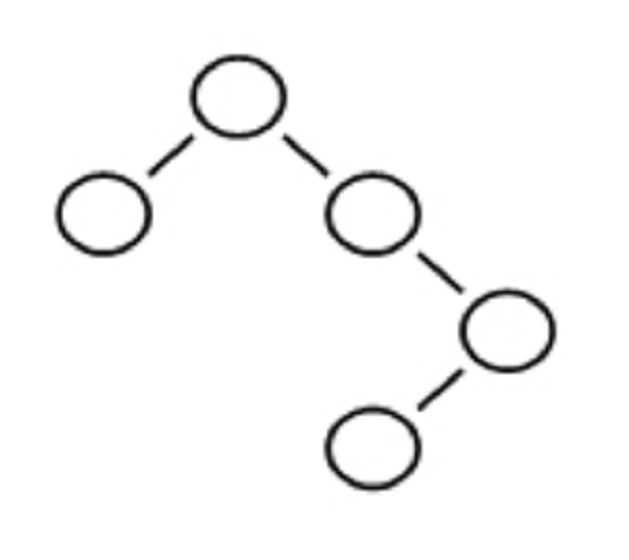
\includegraphics[scale=1]{B.PNG}}
 \end{figure}
 \begin{figure}[H]
     \centering
    \subfigure[C]{
       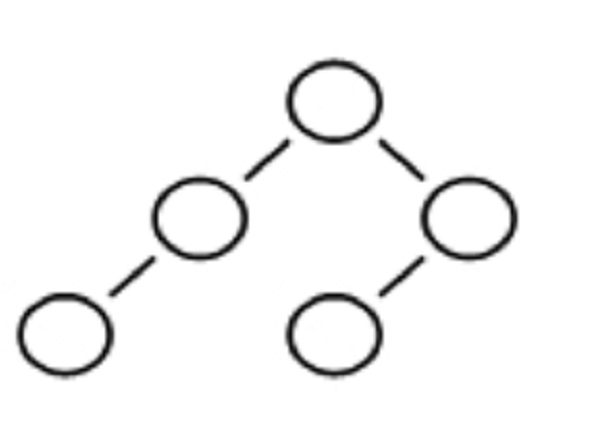
\includegraphics[scale=1]{C.PNG}}
     \hspace{0.5in} 
    \subfigure[D]{
       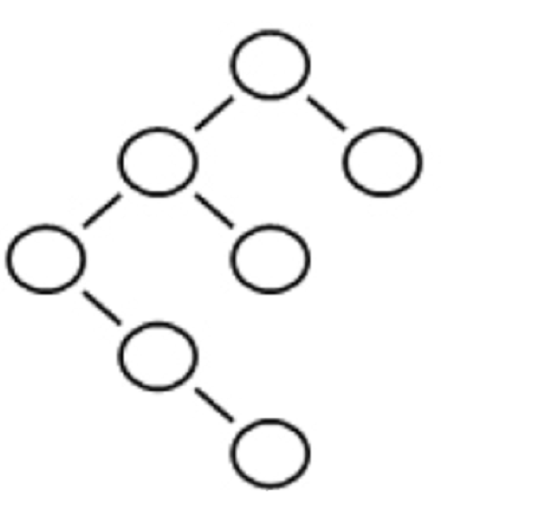
\includegraphics[scale=1]{D.PNG}}
 \end{figure}
\begin{solution}
    
\end{solution}
\item Insert 1, 2, 3, 6, 5, 4 sequentially into an initially empty AVL tree, which of the following rotations will occur?
\begin{solution}
    
\end{solution}
\item Suppose an AVL tree of height N has at least A (n) nodes. 
Then, write A recursive formula to show how A (n) is generated.
\begin{solution}

\end{solution}
\item According to the above formula, we can get the following formula:
\begin{equation}
    A(n)=\frac{(2+\sqrt{5})\left(\frac{1+\sqrt{5}}{2}\right)^{n}-(2-\sqrt{5})\left(\frac{1-\sqrt{5}}{2}\right)^{n}}{\sqrt{5}}-1
\end{equation}
For large n we have the following approximation:
\begin{equation}
    \mathrm{n} \sim \frac{1}{\log \left(\frac{1+\sqrt{5}}{2}\right)} \log A(n) \sim 1.44 \log A(n)
\end{equation}
Please think about how the formula (1) is obtained.
\begin{solution}
    \\ \hspace*{\fill} \\
    \\ \hspace*{\fill} \\
\end{solution}
\item Use the top two equations to answer the following questions:
If the depth of the AVL tree is 6, what is the minimum number of nodes of the tree?
\begin{solution}
    
\end{solution}
What is the maximum depth of an AVL tree with 12 nodes?
\begin{solution}
   
\end{solution}
\end{enumerate}
%%%%%%%%%%%%%%%%%%%%%%%%%%%%%%%%%%%%%%%%%%%%%%%%%%%%%%%%%%%%%%%%%%%%%%%%%%%%%%%%%%%%%%%%%%%
\section{RB tree}
\subsection{Path length}
Among the path from Node x to leaf node, is there one path that is greater than the double of that of another path? Prove your conclusion.
\begin{solution}
    \\ \hspace*{\fill} \\
    \\ \hspace*{\fill} \\

\end{solution}
   
\subsection{Init}
Init a tree by $insert$ function. How many nodes are needed to ensure that there is a red node in the tree?
\begin{solution}
    \\ \hspace*{\fill} \\
    \\ \hspace*{\fill} \\
   
\end{solution}
\subsection{Root node}
Why the root node must be black? What will happen is root node is red?
\begin{solution}
    \\ \hspace*{\fill} \\
    \\ \hspace*{\fill} \\

\end{solution}
    
\subsection{Insert}
Draw the tree after insert 2,4,3,0,5 into the tree. There is one node (Black 1) in the tree at first.
\begin{solution}
    \\ \hspace*{\fill} \\
    \\ \hspace*{\fill} \\
    
\end{solution}

%%%%%%%%%%%%%%%%%%%%%%%%%%%%%%%%%%%%%%%%%%%%%%%%%%%%%%%%%%%%%%%%%%%%%%%%%%%%%%%%%%%%%%%%%%%
\section{BST}
    \subsection{New Edge in BST}
    Suppose we now have a tree. Try to prove that a new edge is added, there should be a cycle.\par 
    \begin{solution}
        \\ \hspace*{\fill} \\
        \\ \hspace*{\fill} \\
       
    \end{solution}
    \subsection{K's smallest number}
    Suppose we have a binary search tree. Output the k's smallest number of the tree. Write the pseudocode or C++ code under. You can just call the root of the tree $root$\par 
    The difinition of the node and function in C++ is shown below:\par 
    \begin{lstlisting}[language = C++]
    Struct TreeNode{
       int data;
       TreeNode* left, right; 
    }
    int kthSmallest(TreeNode* root, int k)
    \end{lstlisting}
    
    \begin{solution}
        \\ \hspace*{\fill} \\
        \\ \hspace*{\fill} \\
       
    \end{solution}
%%%%%%%%%%%%%%%%%%%%%%%%%%%%%%%%%%%%%%%%%%%%%%%%%%%%%%%%%%%%%%%%%%%%%%%%%%%%%%%%%%%%%%%%%%%

\section{Pyramid of numbers}
A number pyramid is an isosceles triangle of numbers with a total of n numbers in the NTH row (as shown below). 
The Blue Tiger needs to find a path from the vertex to the edge that maximizes the sum of numbers passed, 
each step leading to the lower left or lower right of the current point.
\begin{figure*}[htbp]
    \centering
    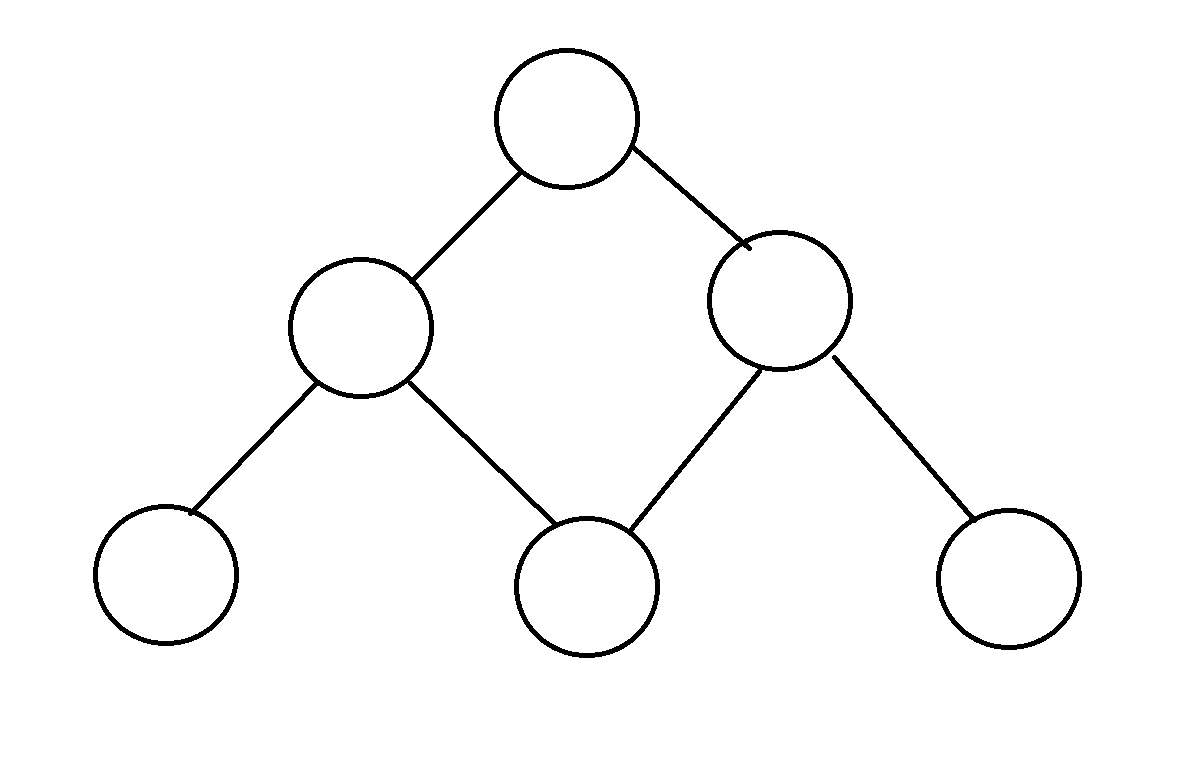
\includegraphics[scale = 1]{number.png}
\end{figure*}
\subsection{Search}
Blue Tiger first considered the idea of brute force solution, 
starting point and end point clear, clear rules of the way, so it can be solved by searching.
Please complete the code he didn't finish and write down the time complexity of the method.
\begin{lstlisting}
    int n, ans , A[100000][100000] 
    //n is the number of row, ans is the final answer, A store the number pramid.
    void Dfs(int x, int y, int curr){
        if (x==n){
            if (       ) ans = curr;
            return ;
        }
        // Add code here if necessary


    }
    int main(){
        cin >> n
        for (int i =0; i<n; i++){
            for (int j=0; j<i; j++){
                cin >> A[i][j];
            }
        }
        ans=0;
        Dfs(0,0,A[0][0]);
        cout << ans << endl;
        return 0;
    }
\end{lstlisting}
\begin{solution}
    \\ \hspace*{\fill} \\
    \\ \hspace*{\fill} \\
    \\ \hspace*{\fill} \\
    \\ \hspace*{\fill} \\
    \\ \hspace*{\fill} \\
    \\ \hspace*{\fill} \\
    \\ \hspace*{\fill} \\
    \\ \hspace*{\fill} \\
   
\end{solution}
\subsection{Whether the greedy algorithm works}
Blue Tiger found the time complexity of the above method very high and decided to make some optimizations. 
He first came up with a greedy algorithm for optimization. 
Greedy algorithm is a method to obtain the global optimal solution by considering the local optimal solution. 
In this problem, it can be interpreted as choosing to go to the position with the larger number in the lower left or lower right at the current position.
But that approach turned out to be wrong. Please find a case where the algorithm is incorrect.
\begin{solution}
    \\ \hspace*{\fill} \\
    \\ \hspace*{\fill} \\
    \\ \hspace*{\fill} \\
    \\ \hspace*{\fill} \\
    \\ \hspace*{\fill} \\
    \\ \hspace*{\fill} \\
    \\ \hspace*{\fill} \\
    \\ \hspace*{\fill} \\
    
\end{solution}
\subsection{Memorized search}
The Blue Tiger found that in the first question, multiple paths to each point were searched repeatedly. 
For example, from (0,0) to (1,2) there's a left path and a right path; So every path from (1,2) to the destination is searched twice. 
Therefore, the blue Tiger chose the memory search method to optimize. Please complete the code below and write the time complexity of the algorithm.
\begin{lstlisting}
    int n, A[100000][100000] ,F[100000][100000]
    void Dfs(int x, int y){
        if (F[i][j]==-1){
            if(x==n) F[x][y]=A[x][y];
            else {
                // Add code here if necessary


            }
        }
        // Add code here if necessary

        return F[x][y];
    }
    int main(){
        cin >> n
        for (int i =0; i<n; i++){
            for (int j=0; j<i; j++){
                cin >> A[i][j];
                F[i][j]=-1;
            }
        }
        // Add code here if necessary

        cout <<      << endl;
        return 0;
    }
\end{lstlisting}
\begin{solution}
    \\ \hspace*{\fill} \\
    \\ \hspace*{\fill} \\
    \\ \hspace*{\fill} \\
    \\ \hspace*{\fill} \\
    \\ \hspace*{\fill} \\
    \\ \hspace*{\fill} \\
    \\ \hspace*{\fill} \\
    \\ \hspace*{\fill} \\
\end{solution}
\subsection{Dynamic programming}
Blue Tiger found that the memory search algorithm is already a dynamic programming algorithm in nature. 
So he tried to solve the problem using dynamic programming.
\subsubsection{Boundary conditions and state transition equations}
Please write down the boundary conditions and the state transition equation for this problem.
\begin{solution}
    \\ \hspace*{\fill} \\
    \\ \hspace*{\fill} \\
    \\ \hspace*{\fill} \\
    \\ \hspace*{\fill} \\
    \\ \hspace*{\fill} \\
    \\ \hspace*{\fill} \\
    \\ \hspace*{\fill} \\
    \\ \hspace*{\fill} \\
\end{solution}
\subsubsection{Program implementation}
Please help Blue Tiger complete the dynamic programming procedure.
\begin{solution}
    \\ \hspace*{\fill} \\
    \\ \hspace*{\fill} \\
    \\ \hspace*{\fill} \\
    \\ \hspace*{\fill} \\
    \\ \hspace*{\fill} \\
    \\ \hspace*{\fill} \\
    \\ \hspace*{\fill} \\
    \\ \hspace*{\fill} \\
\end{solution}
%%%%%%%%%%%%%%%%%%%%%%%%%%%%%%%%%%%%%%%%%%%%%%%%%%%%%%%%%%%%%%%%%%%%%%%%%%%%%%%%%%%%%%%%%%%

\section{0-1 Knapsack problems}
Knapsack problem is a combinatorial optimization problem: given $n$ items,
each with a weight $w_i > 0$ and a value $v_i$, determine the number
of each item to include in a collection so that the total weight is less than or
equal to a given capacity $W$ and the total value is as large as possible.

\subsection{Basic solution}

For 0-1 problem, each item can be decided to be put into the knapsack once or not.
Please fill in the missing code below.

\begin{lstlisting}
int knapsack(const vector<int> &w, const vector<int> &v){
    vector<vector<int>> dp(n + 1, vector<int>(W + 1, 0));
    for (int i = 1; i <= n; ++i){
        for (int j = 1; j <= W; ++j){
            // Add code here
            dp[i][j] = dp[i - 1][j];
            if (w[i - 1] <= j) {
                dp[i][j] = max(dp[i][j], dp[i - 1][j - w[i]] + v[i]);
            }
        }
    }
    return dp[n][W]// Add code here
}
\end{lstlisting}
What is the space-complexity?
\begin{solution}
    \\ \hspace*{\fill} \\
    \\ \hspace*{\fill} \\
    \\ \hspace*{\fill} \\
    \\ \hspace*{\fill} \\
    \\ \hspace*{\fill} \\
    \\ \hspace*{\fill} \\
    \\ \hspace*{\fill} \\
    \\ \hspace*{\fill} \\

\end{solution}
Can we exchange line 3 and 4?
\begin{solution}
    \\ \hspace*{\fill} \\
    \\ \hspace*{\fill} \\
    \\ \hspace*{\fill} \\
    \\ \hspace*{\fill} \\
    \\ \hspace*{\fill} \\
    \\ \hspace*{\fill} \\
    \\ \hspace*{\fill} \\
    \\ \hspace*{\fill} \\

\end{solution}

\subsection{Can we do better?}


Can we achieve a better space-complexity? If so, explain your optimizations and modify code and
the improved space-complexity. Otherwise, explain in one sentence why we cannot improve space-complexity
(Don't change line 3 and 4).
\begin{solution}
    \\ \hspace*{\fill} \\
    \\ \hspace*{\fill} \\
    \\ \hspace*{\fill} \\
    \\ \hspace*{\fill} \\
    \\ \hspace*{\fill} \\
    \\ \hspace*{\fill} \\
    \\ \hspace*{\fill} \\
    \\ \hspace*{\fill} \\
    
\end{solution}

\subsection{Even better?}
Actually we can use even more optimized space from dynamic programming (Hint: you
can change the loop for your own sake). Write your code below.

\begin{solution}
    \\ \hspace*{\fill} \\
    \\ \hspace*{\fill} \\
    \\ \hspace*{\fill} \\
    \\ \hspace*{\fill} \\
    \\ \hspace*{\fill} \\
    \\ \hspace*{\fill} \\
    \\ \hspace*{\fill} \\
    \\ \hspace*{\fill} \\

\end{solution}

Can we exchange the two loops?
\begin{solution}
    \\ \hspace*{\fill} \\
    \\ \hspace*{\fill} \\
    \\ \hspace*{\fill} \\
    \\ \hspace*{\fill} \\
    \\ \hspace*{\fill} \\
    \\ \hspace*{\fill} \\
    \\ \hspace*{\fill} \\
    \\ \hspace*{\fill} \\
   
\end{solution}

What is the time complexity of the algorithm?
\begin{solution}
    \\ \hspace*{\fill} \\
    \\ \hspace*{\fill} \\
    \\ \hspace*{\fill} \\
    \\ \hspace*{\fill} \\
    \\ \hspace*{\fill} \\
    \\ \hspace*{\fill} \\
    \\ \hspace*{\fill} \\
    \\ \hspace*{\fill} \\
    
\end{solution}


\end{document}